% Error Anatomy and Stability of Structural Concept Formation
\documentclass[conference]{IEEEtran}

\usepackage[T1]{fontenc}
\usepackage[utf8]{inputenc}
\usepackage{graphicx}
\usepackage{amsmath,amssymb}
\usepackage{booktabs}
\usepackage{multirow}
\usepackage{xcolor}
\usepackage{url}
\usepackage[hidelinks]{hyperref}

\newcommand{\cid}[1]{\texttt{#1}}   % concept identifiers: \cid{2\_2}

\begin{document}

\title{Error Anatomy and Stability of Structural Concept Formation\\
in a Graph-Based Classifier Without Backpropagation}

\author{
\IEEEauthorblockN{Mykyta Lapin}
\IEEEauthorblockA{Department of System Analysis and Information-Analytical Technologies,\\
National Technical University ``Kharkiv Polytechnic Institute'', Kharkiv, Ukraine\\
Mykyta.Lapin@cit.khpi.edu.ua}
}
% ORCID (verified 2026-04-27, see project canonical table):
%   Lapin 0009-0003-6307-1172

\maketitle

\begin{abstract}
Structural classifiers that form explicit graph concepts promise
interpretable decisions, but their failure modes and the stability of
their concept formation receive little of the scrutiny given to accuracy
benchmarks. We study both questions on a non-backpropagation classifier
that converts images into attributed bipartite skeleton graphs, forms
per-class \emph{concept attractors} by iterative critical-point reduction,
and decides by winner-take-all competition over graph-similarity scores,
reaching 91.13\% accuracy on classified images of the complete-contour
MNIST test subset (90.90\% counting pipeline failures). The dominant
confusion, digit 2 predicted as 7, traces to the representation front end:
at the run's binarization threshold, the topological hole of the digit's
lower-left loop is already missing from the binarized image in 110 of 111
cases --- the loop is drawn open in the handwriting, or its small interior
is flooded by a thick stroke. Ablations exclude the complexity pre-filter
and the ranking prior as remedies; whether the similarity function itself
should still separate the impoverished graphs remains an open design
question. Five exploratory stability studies then characterize formation:
node counts are invariant to sample-presentation order for three probed
concepts, node and edge counts freeze within tens of samples for all thirteen
concepts while the parameter envelope keeps widening, the concepts
generalize to uncurated MNIST
splits at reduced accuracy, and concepts store 91.9$\times$ fewer nodes
than the training graphs they consume. For this dominant confusion the
bottleneck sits in the image-to-graph front end, upstream of concept
formation, and the concepts the system learns are compact and largely
reproducible.
\end{abstract}

\begin{IEEEkeywords}
structural pattern recognition, graph edit distance, concept formation,
few-shot learning, skeletonization, explainable AI, MNIST
\end{IEEEkeywords}

% =========================================================================
\section{Introduction}
% =========================================================================

Most modern image classifiers optimize millions of weights by
backpropagation and explain their decisions only post hoc. An alternative
line of work encodes images as attributed graphs and learns explicit
structural \emph{concepts} whose nodes, edges, and parameter ranges remain
human-readable~\cite{parzhyn2013principles,parzhyn2025architecture,lapin2025fewshot}.
In our system, an image is skeletonized into a bipartite graph of critical
points and connecting segments, per-class concepts are formed by iterative
graph reduction without gradient descent, and classification is a
winner-take-all (WTA) competition in which concepts are scored by an
attribute-weighted graph-similarity measure derived from graph edit
distance (GED)~\cite{bunke1983inexact,riesen2009approx} and ranked by that
score plus a prior favoring the more complex concept. The approach was
introduced in~\cite{lapin2025fewshot}, which reports $\approx$82\%
accuracy from five to six samples per class; in the
configuration studied here it reaches 91.13\% accuracy on the
complete-contour subset of the MNIST test
set~\cite{lecun1998gradient} with only 13 concepts formed from 869
training samples, which derive from 85 unique source images, and every
concept parameter inspectable.

Accuracy alone, however, says little about why such a system fails
when it fails, and whether the concepts it forms are stable artifacts or
accidents of training order and sample choice. Both questions matter more
for structural classifiers than for weight-based ones precisely because
the internal representation claims semantic meaning: a concept that
changes with presentation order, or an error whose cause cannot be located
in the pipeline, would undermine the interpretability argument itself.

This paper answers both questions empirically. Our contributions are:

\begin{enumerate}
\item \textbf{An anatomy of the dominant error.} The most frequent
confusion of the baseline (true digit 2 predicted as 7; 111 of 792
failures, 14.0\% of the error mass)
superficially contradicts the WTA design: the concept for class~2 is
more complex than the one for class~7, so it should win when it
matches. We trace all 111 cases through the production scoring code,
localize the anchor-point loss stage by stage (binarized mask: 110 of 111;
vectorization: 1 of 111; reduction and inference: 0), exclude the
complexity pre-filter and the ranking prior by direct ablation, and verify
the cost implementation by replay; the suitability of the similarity
projection itself remains open (Section~\ref{sec:postmortem}).
\item \textbf{Five exploratory stability studies of concept formation},
covering generalization to other MNIST splits, sample-order dependence
(three concepts, ten orders), sample-count dependence (three draws per
condition), reduction convergence, and storage compression, each with its
scope stated (Section~\ref{sec:studies}).
\item \textbf{A diagnosis with design consequences}: the dominant error
cluster originates in the representation front end and resists every
parameter-level downstream repair we tested, while the
formation process itself is largely order-invariant, freezes node and edge
counts after few samples in all thirteen concepts, and compresses
input structure by 91.9$\times$ in nodes and 50.6$\times$ in stored values
under the counting convention of Section~\ref{sec:compression}
(Section~\ref{sec:discussion}).
\end{enumerate}

All analyses run on the production code paths, with no re-implemented
scoring.

% =========================================================================
\section{Related Work}
\label{sec:related}
% =========================================================================

\textbf{Graph matching and GED.} Pattern recognition has used graphs as a
structural representation since the late
1970s~\cite{conte2004thirty}, with graph edit distance providing the
standard error-tolerant similarity measure since Bunke and
Allermann~\cite{bunke1983inexact}. Because exact GED is NP-hard, practical
systems rely on approximations such as bipartite
matching~\cite{riesen2007bipartite} and its journal
refinement~\cite{riesen2009approx}. Our classifier uses an
attribute-weighted, GED-derived similarity as its scorer; this paper
contributes a measured account of how a complete GED-based classifier
fails and how stable its learned structures are --- an analysis the
graph-matching literature rarely applies to end-to-end systems.

\textbf{Learning without backpropagation.} Interest in alternatives to
end-to-end gradient descent ranges from topology-learning networks such as
Growing Neural Gas~\cite{fritzke1995growing} to Hinton's forward-forward
algorithm~\cite{hinton2022forward}. The system studied here descends from
the modal-vector theory of formal intelligence
systems~\cite{parzhyn2013principles,parzhyn2025architecture} and its
energy formulation~\cite{parzhyn2025energy}: concepts are formed by
deterministic graph reduction rather than weight updates. The
classifier itself was introduced in~\cite{lapin2025fewshot}, which reports
an earlier, smaller-scale result; the present paper analyzes the
full baseline and supplies the missing error anatomy and stability
evidence.

\textbf{Few-shot and prototype-based learning.} Learning a class from
tens of examples is the goal of few-shot methods such as prototypical
networks~\cite{snell2017prototypical} and model-agnostic
meta-learning~\cite{finn2017model}, which position class prototypes in a
\emph{learned embedding space}. Lake et al.~\cite{lake2015human} showed
that compositional, generative structure enables human-level one-shot
character learning. Our concepts play the prototype role but remain
explicit attributed graphs whose every node and range is inspectable ---
closer in spirit to~\cite{lake2015human} than to embedding-based
prototypes.

\textbf{Interpretability and error accountability.} Rudin's argument for
inherently interpretable models over post-hoc
explanations~\cite{rudin2019stop} motivates our evaluation standard: a
model whose internal representation claims semantic meaning must also
support locating the cause of each error and showing that its learned
structures survive changes in training order. The present work
operationalizes that standard for a structural classifier.

% =========================================================================
\section{System Overview}
\label{sec:system}
% =========================================================================

We summarize the pipeline only to the depth needed for the analyses; the
representation and formation method are described
in~\cite{lapin2025fewshot,parzhyn2025energy}.

\subsection{Image-to-graph construction}

An input image is binarized (intensity threshold 110--180, adaptively
retried on disconnection), thinned to a one-pixel
skeleton~\cite{zhang1984fast}, and approximated by a Growing Neural Gas
network~\cite{fritzke1995growing} whose output polyline is simplified with
the Ramer--Douglas--Peucker algorithm~\cite{douglas1973algorithms}. The
result is an attributed \emph{bipartite} graph: \emph{Point} nodes
(endpoints, corners, junctions, a start point) alternate with \emph{Vector}
nodes (line segments carrying length, direction, and quadrant attributes).
Node coordinates are normalized to a centered $[-1,1]$ system for scale
and translation invariance. We define the \emph{complexity} of a graph as
its total number of nodes plus edges.

\subsection{Concept formation}

For each class, training graphs are merged one at a time into a concept by
critical-point reduction: shared topology is retained, instance-specific
branches are reduced, and each surviving node accumulates per-feature
\emph{ranges} (envelopes) instead of point values. The first sample seeds
the concept; formation is incremental and uses no gradient
signal. A class may yield more than one concept (e.g.\ two stylistic
variants of the digit); the baseline uses 13 concepts for 10 classes,
formed from 869 pre-augmented training samples. Those 869 samples come from
85 unique source images; the other 784 are geometric variants generated
offline from them, five to ten variants per source.

\subsection{Classification}

Classification runs three stages before a winner is picked. A
\emph{complexity pre-filter} first discards every concept whose complexity
exceeds the image complexity, before any comparison runs, on the rationale
that a simple image cannot instantiate a more complex concept. Each
surviving concept is then prepared against its own isolated copy of the
image graph: the concept's learned centroid direction and expected start
degree anchor a concept-specific start point in the image, and the image
graph is reduced by endpoint, intersection, and corner-point operations
until its critical-point structure is isomorphic to the concept's. Every
concept therefore scores against a differently anchored and differently
reduced version of the image. Preparation also enforces \emph{structural
compatibility gates} for pairings the representation cannot support, such as
a concept containing intersection points matched against an image that has
none, or a concept with more corner points than the image. A concept that
hits a gate, or that cannot be reduced to isomorphism within the iteration
budget, receives no similarity score at all and ranks below every scored
concept; that outcome differs from scoring low.

The prepared pair is then scored by a GED-derived similarity over 13 node
features. Substitution costs are attribute-weighted, each feature weighted
inversely to the width of the concept's learned interval
($\varepsilon = 0.1$), so a narrow diagnostic range counts for more than a
wide one. Edit costs are asymmetric: inserting a concept node the image
lacks costs 6.0, deleting an image node the concept does not account for
costs 0.25, and edge insertion is free, which biases the measure toward
subgraph containment --- whether the image contains the concept. The total
edit cost $c$ becomes a similarity $s = 1 - c/(c + \max(n_1, n_2))$
normalized by the larger graph, with $n_i$ counting nodes plus edges. The
winner-take-all step finally ranks the scored concepts by the adjusted score
$\hat{s} = s + \lambda \log_2 C$ with $\lambda = 0.10$, where $C$ is the
concept's complexity. This prior states the design intent that among
concepts which match adequately, the more complex one should win: a small
concept matches an arbitrary graph more easily, so its similarity carries
less evidence. The concept at the top of this ranking is the winner and its
class is the prediction.

\subsection{Baseline}
\label{sec:baseline}

The reference run\footnote{Run \texttt{run\_20260630\_235356}; artifacts
(configuration, metrics, confusion matrix, per-image errors, concept
graphs) are archived with the code.} evaluates the full \emph{complete-only}
MNIST test subset: 8{,}704 of the 10{,}000 test images whose contours are
complete (unbroken strokes), a restriction discussed in
Section~\ref{sec:datasets}. The run log records 8{,}707 submissions over
these 8{,}704 images; 22 submissions failed in
skeletonization (dead-letter queue) and 8{,}685 were classified, with
accuracy $91.13\%$, precision $91.92\%$, recall $91.13\%$, and F1
$91.34\%$ over the classified set. Counting every submission in the
denominator yields the end-to-end accuracy $7{,}915/8{,}707 = 90.90\%$.
Throughout the paper we keep both readings apart: \emph{conditional}
accuracy is measured over classified images, \emph{end-to-end} accuracy
over everything submitted.
Figure~\ref{fig:confusion} shows the confusion structure. The largest
confusion pairs are $2{\to}7$ (111), $4{\to}7$ (62), $2{\to}6$ (57),
$4{\to}1$ (52), and $9{\to}4$ (46); classes 2 (215 errors) and 4 (155
errors) dominate the error mass.

\begin{figure}[!t]
\centering

\includegraphics[width=\columnwidth]{figures/confusion_matrix.png}
\caption{Confusion matrix of the 91.13\% baseline on the complete-only
MNIST test subset (8{,}685 classified images, 13 concepts).}
\label{fig:confusion}
\end{figure}

% =========================================================================
\section{Anatomy of the Dominant Error: Why 2s Fall into 7s}
\label{sec:postmortem}
% =========================================================================

The $2{\to}7$ confusion seems to contradict the WTA design. The rich
concept for class~2 (\cid{2\_2}, complexity 24) is far more complex than
the concept for class~7 (\cid{7\_1},
complexity 9, the smallest in the system). Under WTA with a complexity
prior, the rich concept should win whenever it genuinely matches. The
working hypothesis was that \cid{2\_2} never gets to compete: the
image graph loses critical anchor points during construction --- before
reduction --- so the ``2'' arrives at the classifier already impoverished.

We verified this hypothesis on all 111 misclassified images using the
production classification orchestrator and cost functions; the
offline tool reproduced the live prediction for 111/111 images. This
replay runs the current code tree, not a frozen copy of the June baseline:
predicted labels agree in all 111 cases, but raw similarity values drifted
slightly as the scoring code evolved (the primary exemplar's \cid{2\_1}
similarity reads 0.7300 in the run log and 0.7469 in the replay), so the
similarity values reported below are replay values. The
mechanism is two-staged, and both stages share one root cause. Beyond
verifying the hypothesis, we localize the loss stage by stage with a
topological measurement and ablate the two adjustable downstream
mechanisms --- the complexity pre-filter and the ranking prior ---
individually, testing whether either repair short of fixing the input
could flip the outcome.

\subsection{Stage 1: the complexity pre-filter excludes the rich concept}

The median complexity of the 111 misclassified ``2'' graphs is 21
(range 13--29), below the complexity 24 of \cid{2\_2}. Consequently the
pre-filter removes \cid{2\_2} from the competition in 86 of 111
cases (77.5\%). The rich concept does not \emph{lose} the WTA
competition --- it never enters it.

The obvious repair --- remove or soften the pre-filter --- was tested by
direct ablation: we disabled the pre-filter and scored \cid{2\_2} against
all 111 images with the production scoring code. It wins zero of
111 cases, and its raw similarity is $0.0$ in all of them. The reason is
structural: \cid{2\_2} contains the crossing point where
the descending stroke curls back across the base stroke, while no image
graph retains a crossing after degree normalization. The constructed
graphs do contain a degree-3 T-junction node where the descending stroke
meets the base stroke (visible in the second panel of
Figure~\ref{fig:triptych}), but endpoint reduction removes its short
branch and demotes it to a corner point before the gates apply, so the
compatibility gate (``concept
has intersection points but the image does not'') rejects the pairing
before GED optimization runs. The reported $0.0$ is this gate outcome, not
a computed GED score. Impoverished graphs are small, so the
pre-filter is a symptom of the same degradation, not a cause of the
error. Removing it changes nothing.

\subsection{Stage 2: the simplified concept loses on raw similarity}

The simplified concept \cid{2\_1} (complexity 13) is never pre-filtered
--- it competes in all 111 cases --- and loses to \cid{7\_1} on \emph{raw}
similarity in all 111: mean raw similarity 0.673 against 0.813, a mean gap
of 0.140 and a minimum gap of 0.053. In 5 of 111 cases \cid{2\_1} is
additionally zeroed by a second compatibility gate (``concept has more
corner points than the image''). Bucket analysis over all 111 cases
(Table~\ref{tab:buckets}) shows that all 111 errors are
raw-similarity losses (bucket B); there are no cases where no 2-concept
competed at all (bucket A) and no cases where a
2-concept won on raw similarity but lost the final $\lambda$-ranking
(bucket C). The ranking prior is innocent. In the 25 cases where
\cid{2\_2} nominally competed, its similarity was $0.0$ for the same
structural reason as in the ablation above, so it never outscored
\cid{2\_1}.

\begin{table}[!t]
\caption{Anatomy of all 111 $2{\to}7$ errors: buckets, stage
localization of the anchor-point loss, and ablation}
\label{tab:buckets}
\centering
\begin{tabular}{lr}
\toprule
Indicator & Value \\
\midrule
A: no 2-concept in competition & 0 \\
B: 2-concept competes, loses on raw similarity & \textbf{111 (100\%)} \\
C: wins raw similarity, loses $\lambda$-ranking & 0 \\
\midrule
Lower-loop hole absent already in binarized mask & \textbf{110 (99.1\%)} \\
Hole survives to skeleton, lost at vectorization & 1 \\
Anchor points lost at reduction or inference & 0 \\
Final graphs with zero cycles, no crossing point & 111 (100\%) \\
\midrule
\cid{2\_2} excluded by complexity pre-filter & \textbf{86 (77.5\%)} \\
Ablation --- pre-filter removed, \cid{2\_2} wins & 0 of 111 \\
Ablation --- \cid{2\_2} raw similarity & 0.0 in all 111 \\
\cid{2\_2} competed and outscored \cid{2\_1} & 0 of 25 \\
Mean raw similarity, \cid{2\_1} / \cid{7\_1} & 0.673 / 0.813 \\
Raw-similarity gap (mean / min) & 0.140 / 0.053 \\
Image complexity (min / median / max) & 13 / 21 / 29 \\
\bottomrule
\end{tabular}
\end{table}

\subsection{Root cause: the lower-loop hole never reaches the graph}

For each of the 111 images we measured, stage by stage, where the
topological hole of the lower-left loop disappears: holes of the binarized mask
(via its Euler characteristic), cycles of the one-pixel skeleton, and
cycles of the final graph\footnote{Stage measurements use the production
skeletonization code at the run's threshold (110) without the live
pipeline's adaptive threshold retries; final graphs are taken from the
database exactly as the live run produced them.}. The outcome
(Table~\ref{tab:buckets}): in 110 of 111 cases the binarized mask
already contains no hole. Two handwriting mechanisms produce this. Either
the loop is drawn open --- the descending stroke never crosses the base
stroke --- or the loop is filled with ink: its interior encloses only a
few background pixels, so a stroke of ordinary thickness floods it into a
solid blob, the eye ``reads'' a loop into the pixel pattern, but no
topological hole exists, and skeletonizing a solid blob yields a line, not
a cycle (the exemplars of Figures~\ref{fig:construction}
and~\ref{fig:contrast}). In the
single remaining case (\texttt{mnist\_test\_2\_00412}) the mask carries
two measured holes that survive into the skeleton and are
lost during GNG+RDP vectorization; an offline rerun with a different GNG
initialization preserved them, so loss at that stage is stochastic rather
than systematic. No case loses anchor points at reduction or inference:
after graph construction there is nothing left to lose.

All 111 final graphs share the measured invariants of the zigzag concept
\cid{7\_1}: zero cycles and, after degree normalization, no crossing
point. A human judges the pixel image and reads a loop into the ink; the
classifier sees only the graph, which never contained one.

Figure~\ref{fig:construction} traces one canonical exemplar through the
construction stages, and Figure~\ref{fig:triptych} shows the resulting
graph next to the competing concepts.

\begin{figure*}[!t]
\centering
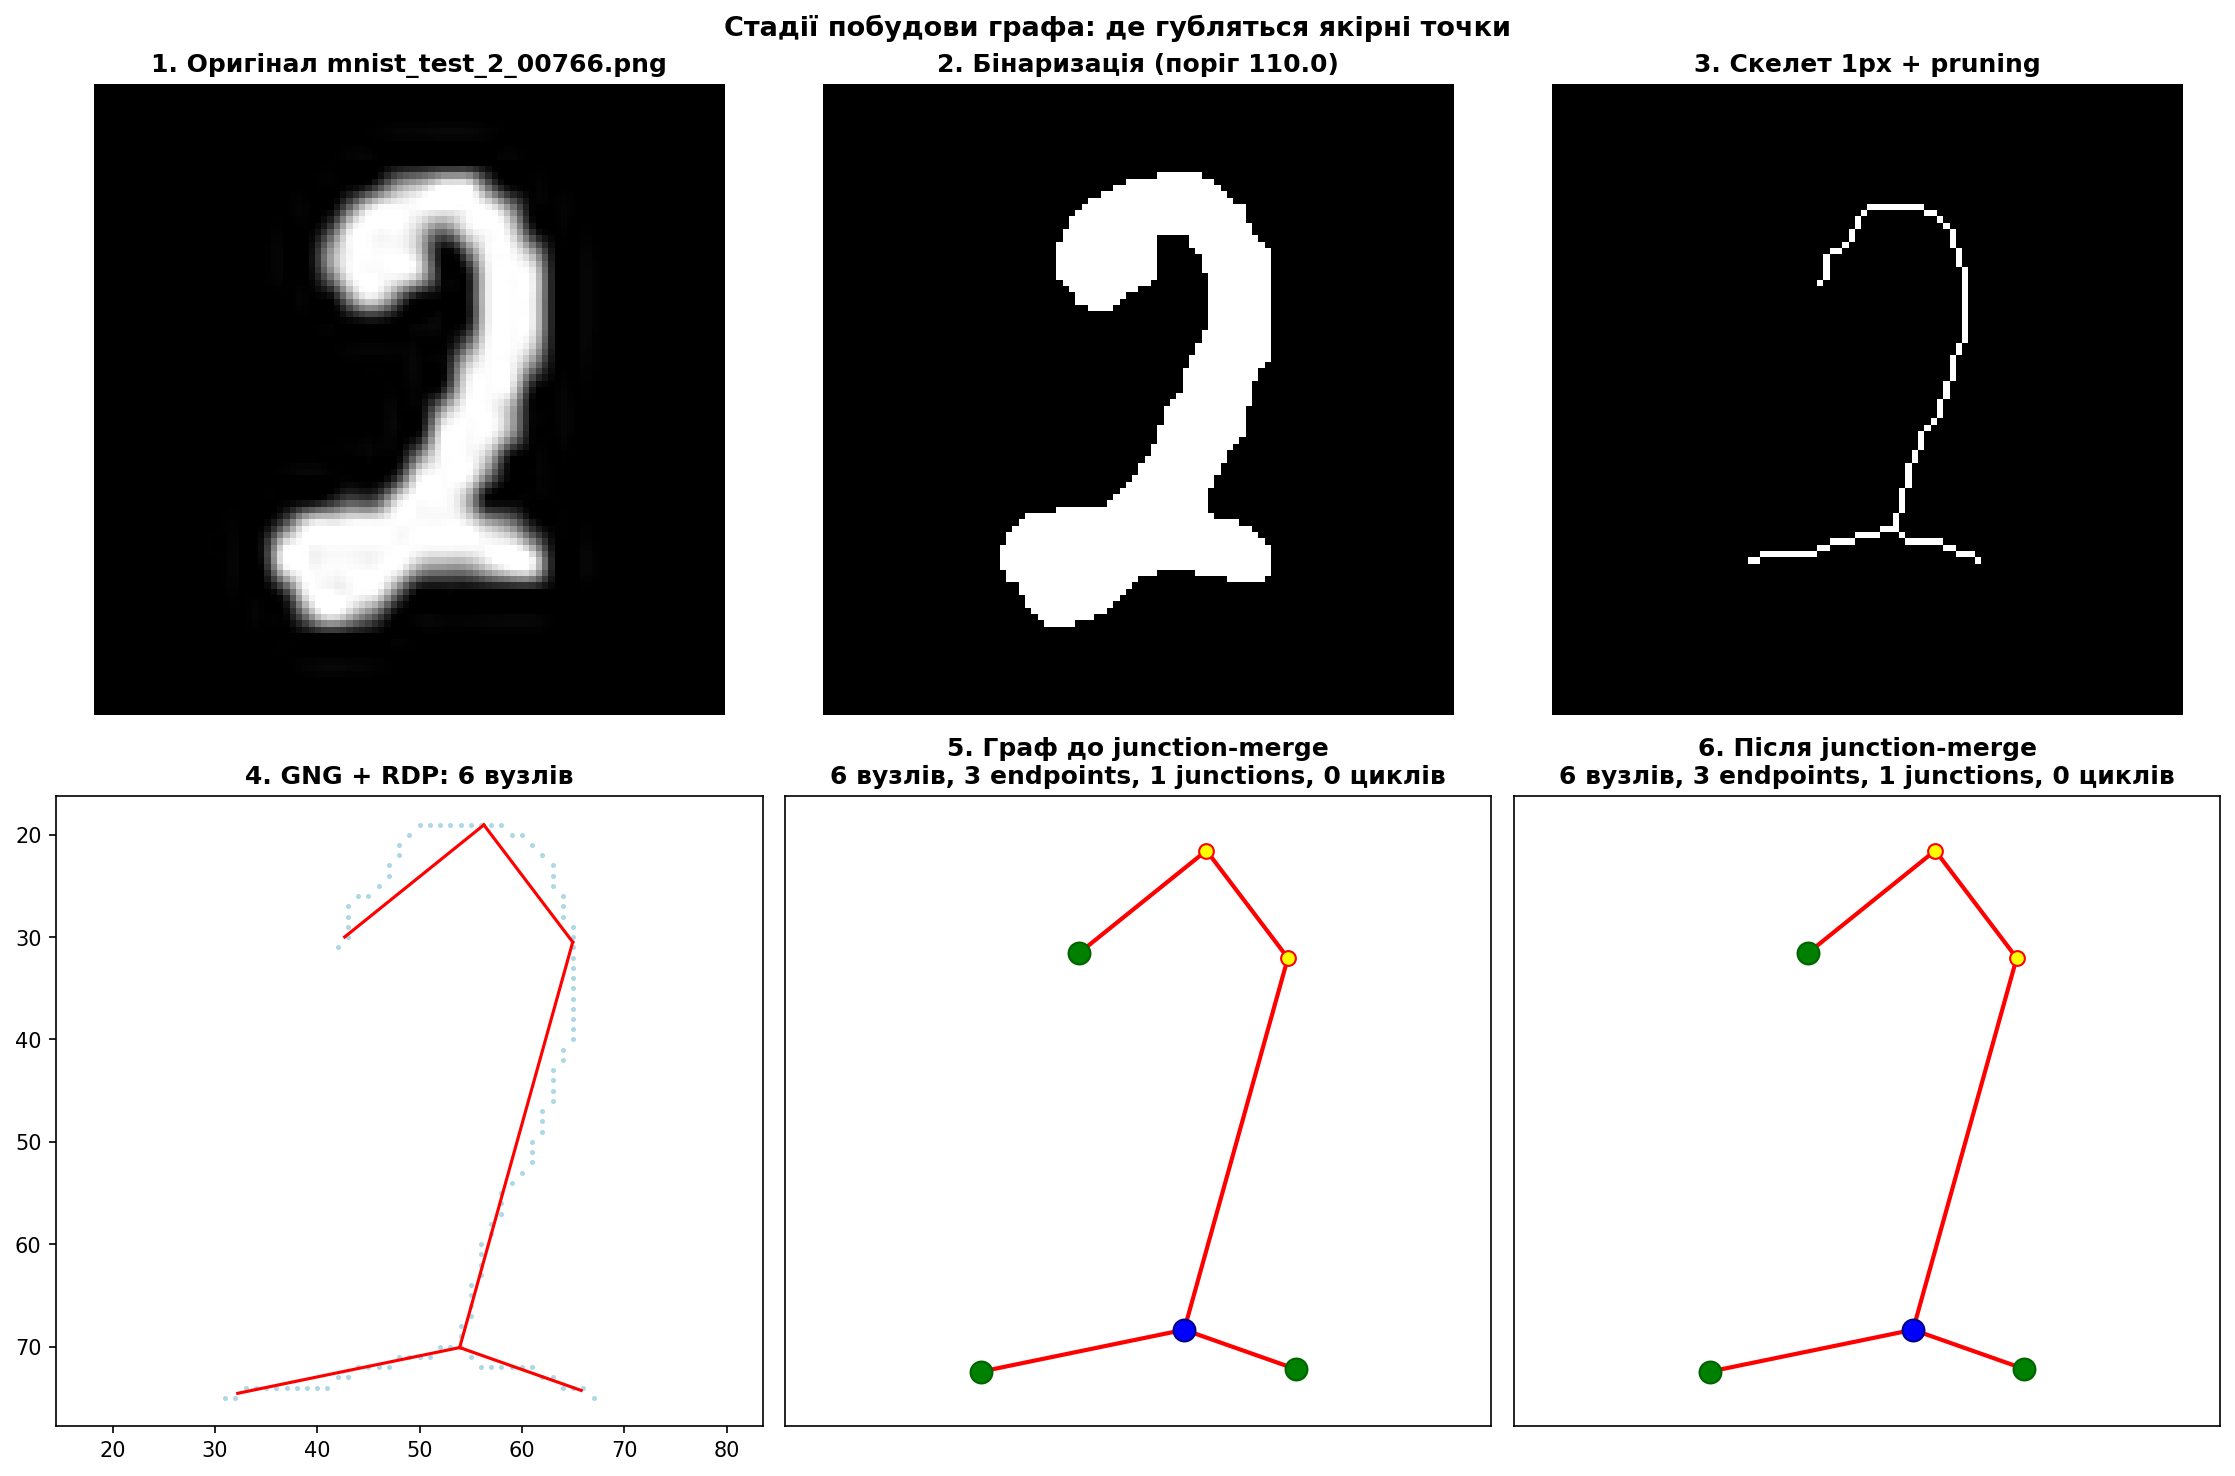
\includegraphics[width=\textwidth]{figures/mnist_test_2_00766_construction.png}
\caption{Construction stages for exemplar \texttt{mnist\_test\_2\_00766}.
The lower-left curl reads as a loop in the grayscale image (panel 1), but
its small interior is flooded into a solid blob in the binarized mask
(threshold 110, panel 2) ---
the mask contains zero topological holes --- so the one-pixel skeleton is
an open hook with zero cycles (panel 3). GNG approximation with RDP
simplification ($\varepsilon = 4.55$) then flattens the hook arc into two
straight segments (panel 4). The intersection anchor point is never
created; the defect precedes any learning step.}
\label{fig:construction}
\end{figure*}

\begin{figure*}[!t]
\centering
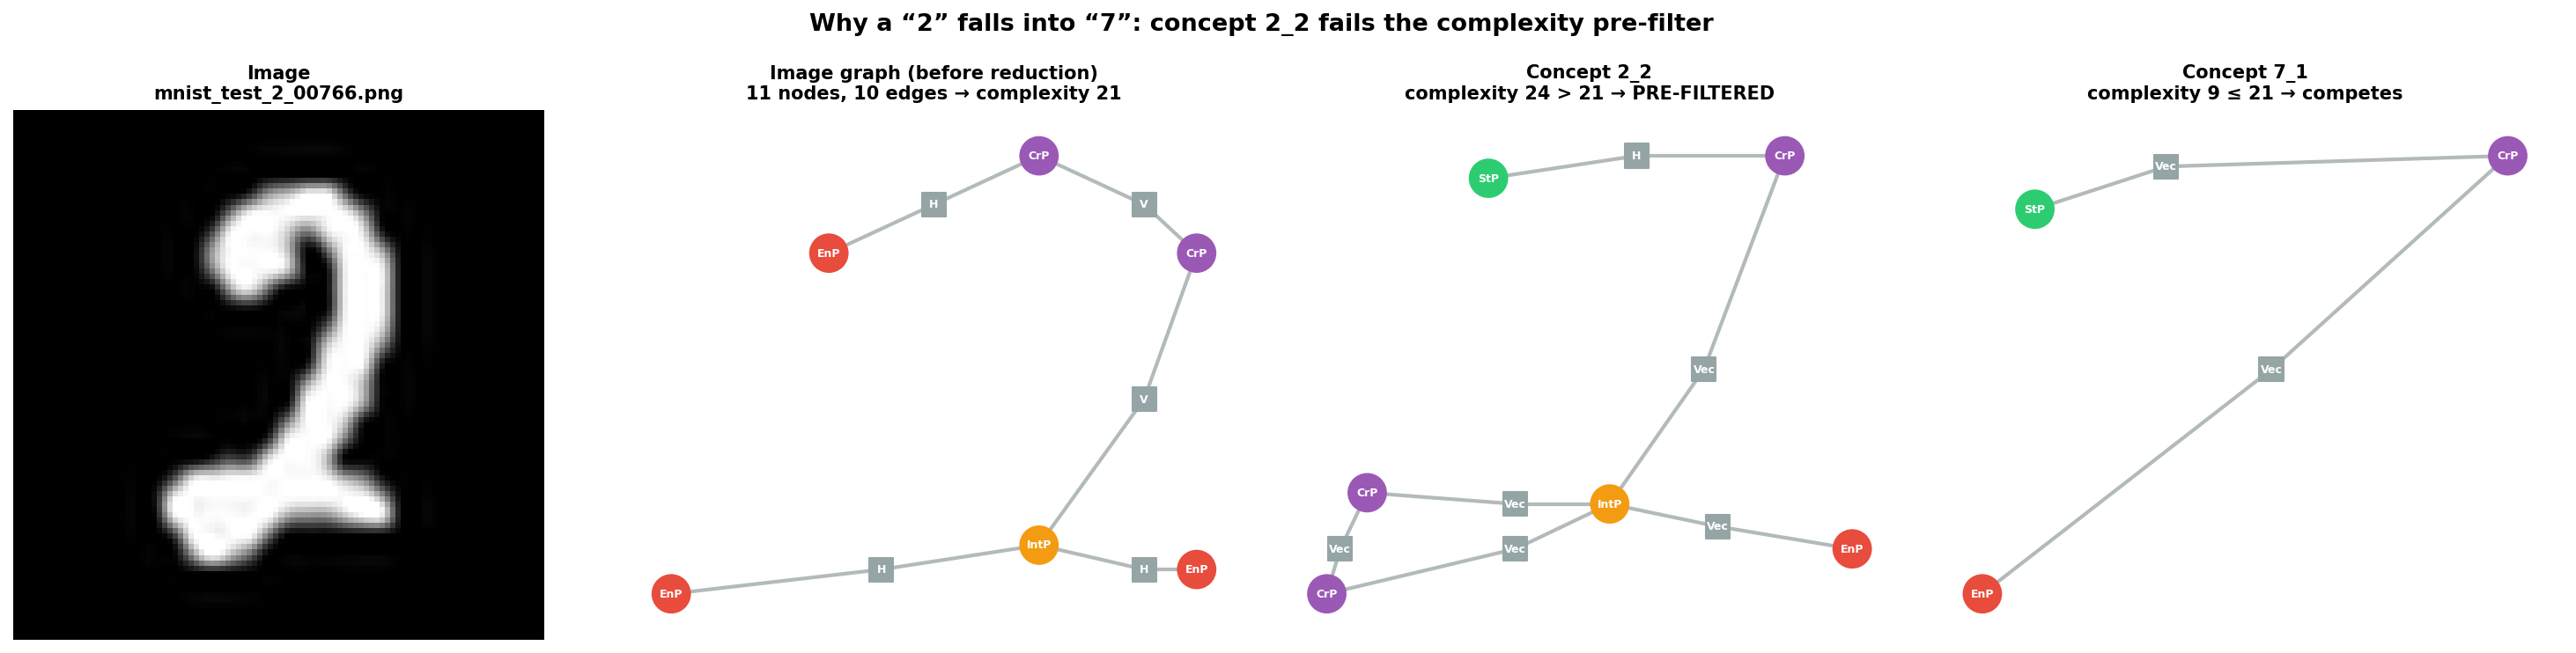
\includegraphics[width=\textwidth]{figures/mnist_test_2_00766_triptych.png}
\caption{Exemplar \texttt{mnist\_test\_2\_00766}, four panels: original
image, constructed image graph before reduction, and the two competing
concepts \cid{2\_2} and \cid{7\_1}. The
image graph has 11 nodes and 10 edges (complexity 21), so concept
\cid{2\_2} (complexity 24) is excluded by the pre-filter; the simplified
\cid{2\_1} then loses to \cid{7\_1} on raw similarity. The T-junction
node shown in the second panel is demoted to a corner point during degree
normalization, before the compatibility gates apply
(Section~\ref{sec:postmortem}).}
\label{fig:triptych}
\end{figure*}

The GNG approximation for this exemplar uses $\approx$35 neurons and
leaves a zigzag-like graph of 6 structural points (3 endpoints, 1
junction, 0 cycles), whose complexity of 21 falls below the 24 of
\cid{2\_2}. Table~\ref{tab:exemplar} gives the production ranking.

\begin{table}[!t]
\caption{Replay ranking for exemplar \texttt{mnist\_test\_2\_00766}
(current code tree, prediction identical to the live run);
the \cid{2\_2} similarity is from the pre-filter-removed ablation}
\label{tab:exemplar}
\centering
\begin{tabular}{lcccc}
\toprule
Concept & Raw sim. & Adjusted & Complexity & In competition \\
\midrule
\cid{7\_1} (winner) & 0.8317 & 1.1487 & 9 & yes \\
\cid{2\_1} & 0.7469 & 1.1169 & 13 & yes \\
\cid{2\_2} & 0.0 & 0.0 & 24 & no (pre-filter) \\
\bottomrule
\end{tabular}
\end{table}

The per-feature breakdown of the \cid{2\_1} comparison shows where
the loss occurs: surviving points sit outside the ranges the concept
learned to expect, with full penalties on three features --- e.g.\
\path{distance_to_centroid} $= 0.558 \notin [0.69, 1.00]$ on the start
point, \path{normalized_x} $= 0.200 \notin [-0.70, 0.10]$ on a corner
point, and \path{length_ratio_to_max} on a segment --- while every
node of \cid{7\_1} substitutes within its intervals. The geometry of the
graph is distorted by the loss of the loop, so the degraded zigzag is
parametrically closer to the tolerances of \cid{7\_1} than to the
intervals of \cid{2\_1}.

The contrast exemplar
(\texttt{mnist\_test\_2\_00984}, Figure~\ref{fig:contrast}) shows the
second mechanism: a flat cursive ``2'' whose lower loop is filled with
ink, so the flooded blob skeletonizes into a zigzag visually close to a
``7''. The median image complexity of 21 against \cid{2\_2}'s 24
identifies graph impoverishment as the dominant factor across the 111
cases.

\begin{figure*}[!t]
\centering
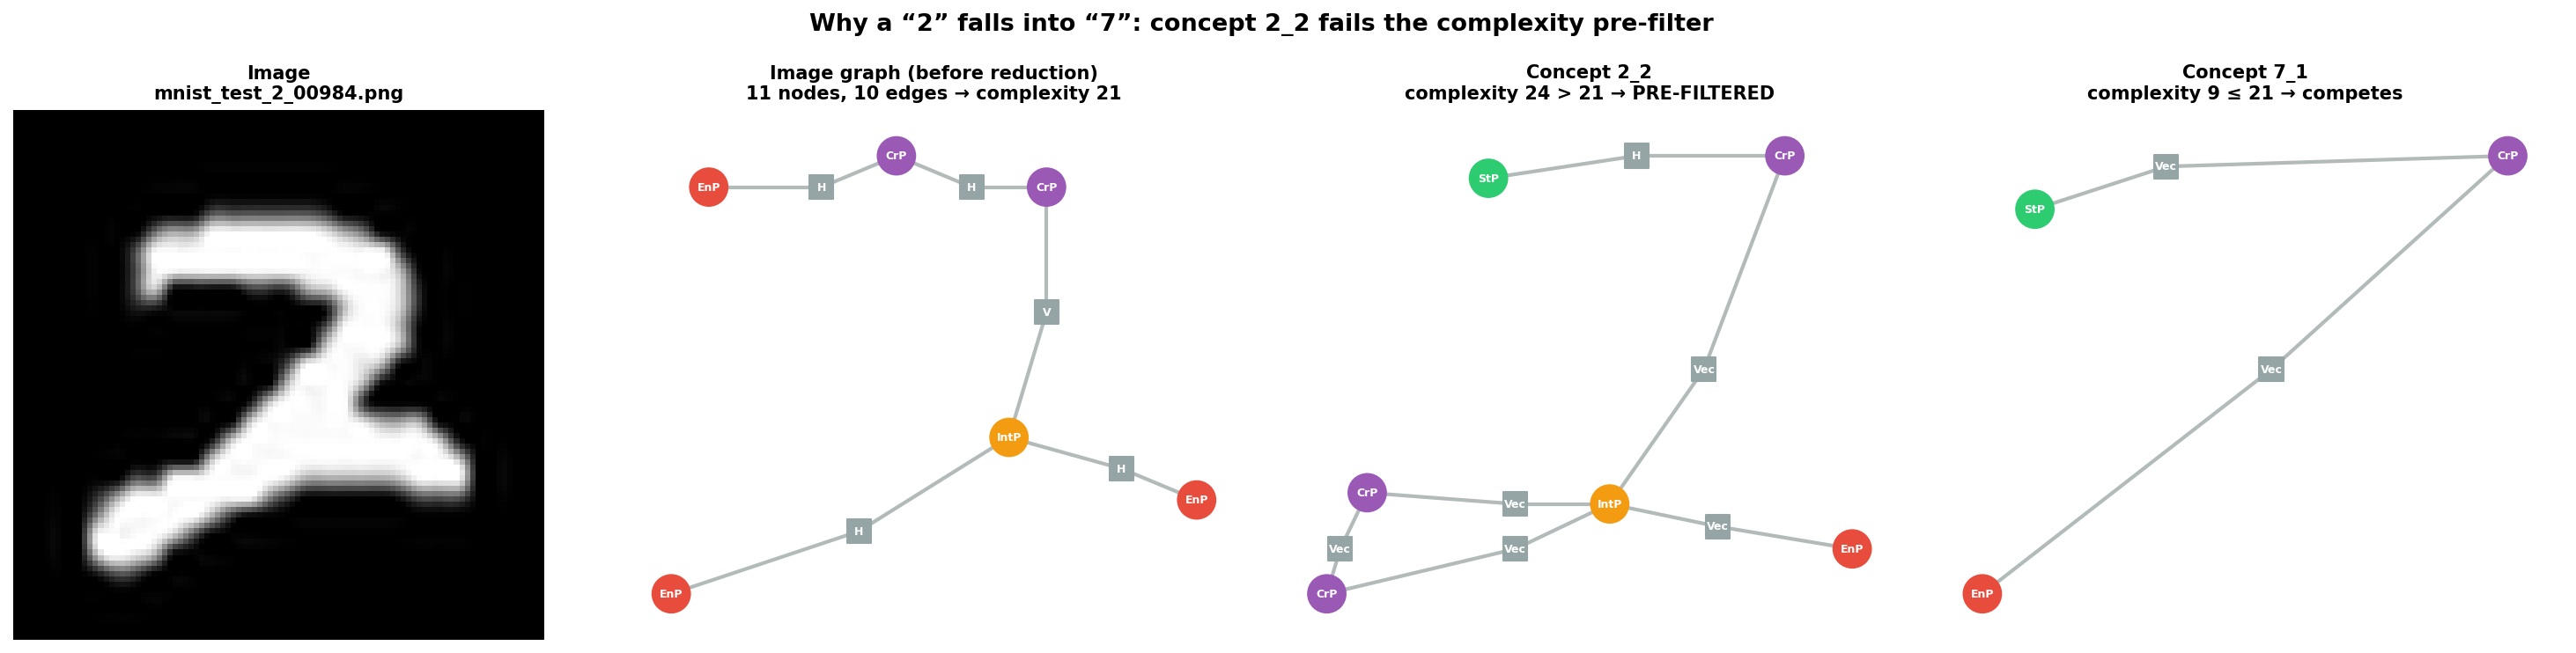
\includegraphics[width=\textwidth]{figures/mnist_test_2_00984_triptych.png}
\caption{Contrast exemplar \texttt{mnist\_test\_2\_00984} (same four-panel
layout as Figure~\ref{fig:triptych}): a flat cursive ``2'' whose lower
loop is filled with ink --- the second handwriting mechanism; the flooded
loop leaves no topological hole, so the graph is an open zigzag.}
\label{fig:contrast}
\end{figure*}

\subsection{What the ablations exclude, and what they do not}

Since every downstream mechanism was suspect, we also checked the scoring
implementation. Decomposing each substitution cost by feature in the
replay reproduces the total cost with a residual of approximately zero.
A self-recognition test scores each concept
against its own typical feature values: all 13 concepts respond with
similarity 1.00, and the parametric layer separates even structurally
isomorphic concept pairs (\cid{2\_1}/\cid{5\_1} and \cid{4\_1}/\cid{9\_2}).
These checks establish that the implementation computes the specified
similarity function consistently; they do not establish that the specified
function is the right projection of graph evidence onto a scalar. The
error graphs retain a short lower-left branch that genuine 7s lack, and
whether a similarity function should exploit it to separate the classes on
the impoverished input is an open question these experiments do not
answer.

\subsection{Consequences}
\label{sec:consequences}

Three design consequences follow, none of which requires hard-coding
concept identities. (i)~Graph construction is the only lever established
by measurement: hole-preserving binarization and skeletonization, and
topology-aware vectorization that controls cycles through GNG, RDP, and
junction merging, would let the lower loop reach the graph, raise image
complexity, return \cid{2\_2} to the competition, and let its intersection
point and cycle-count features discriminate against \cid{7\_1}. One
limit remains: loops filled with ink are not recoverable from the binary
mask alone and would require intensity analysis inside the stroke.
(ii)~The two parameter-level repairs are excluded by experiment:
removing the complexity pre-filter changes nothing (\cid{2\_2}
wins 0 of 111 with similarity 0.0), and the $\lambda$-ranking prior
contributes zero errors. (iii)~The similarity
function itself is the remaining downstream suspect: its implementation is
verified consistent above, but no experiment here tests whether a
different projection could exploit the surviving lower-left branch, so a
scoring redesign stays open as future work.

% =========================================================================
\section{Stability Studies of Concept Formation}
\label{sec:studies}
% =========================================================================

The second question concerns the trustworthiness of the
formation process itself: does the classifier generalize beyond the
curated test subset, and are the concepts it forms stable with respect to
presentation order, sample count, and reduction depth? Five studies
address this. All formation studies run the production formation
code through a seedable offline probe; all evaluation studies run the full
live pipeline.

\subsection{Generalization across MNIST dataset variants}
\label{sec:datasets}

The system is contour-based: a digit drawn with broken strokes yields an
incomplete skeleton that no concept formed from complete contours can
cover. The baseline therefore evaluates the complete-contour subset. To
quantify the cost of this restriction, we evaluated the untouched baseline
concepts on the full MNIST test set (10{,}000 images, no
exclusions) and on the 60{,}000-image training split, whose
completeness labels come from a heuristic
classifier\footnote{The 60k split is labeled by a completeness heuristic,
not manual review; 85 of its images are the unique source images of the
system's training corpus (leakage 0.14\%; the offline-generated variants
are not MNIST members).}. Table~\ref{tab:datasets}
reports the results with the pipeline status made explicit: a submitted
image either receives a prediction, fails into the dead-letter queue
(DLQ), or returns no result at all (the run export records no cause for
the last group). End-to-end accuracy counts every submission in the
denominator; conditional accuracy counts classified images only.

\begin{table*}[!t]
\caption{Accuracy across MNIST dataset variants (baseline concepts, no
retraining), decomposed by pipeline status\textsuperscript{a}}
\label{tab:datasets}
\centering
\begin{tabular}{lrrrrrrrr}
\toprule
Run / split & Submitted & Classified & Completion & Correct &
Conditional & End-to-end & DLQ & Other uncl. \\
\midrule
10k test, all & 10{,}000 & 9{,}942 & 99.42\% & 8{,}221 & 82.69\% & \textbf{82.21\%} & 58 & 0 \\
60k train, all & 60{,}000 & 51{,}045 & 85.08\% & 43{,}172 & 84.58\% & \textbf{71.95\%} & 293 & 8{,}662 \\
70k aggregate & 70{,}000 & 60{,}987 & 87.12\% & 51{,}393 & 84.27\% & \textbf{73.42\%} & 351 & 8{,}662 \\
60k train, complete-only rerun & 45{,}501 & 44{,}812 & 98.49\% & 38{,}469 & 85.85\% & \textbf{84.55\%} & 14 & 675 \\
\bottomrule
\multicolumn{9}{l}{\footnotesize\textsuperscript{a}Completion is
classified/submitted; end-to-end is correct/submitted, so every
unclassified case lowers it.}
\end{tabular}
\end{table*}

Three observations. First, the completeness restriction is load-bearing:
within the 10k run, the complete slice scores $7{,}911/8{,}704 = 90.89\%$
end-to-end while the incomplete slice scores $310/1{,}295 = 23.94\%$,
dragging the no-exclusions figure to 82.21\%. Second, per-slice accuracy
from the 60k all-split run conflates classifier error with pipeline
completion: that run left 8{,}662 submissions without any result
(completion 85.08\%), and its complete slice reads 76.12\% end-to-end,
whereas the dedicated rerun over the same 45{,}501 ``complete'' images
completed 98.49\% and reached 85.85\% conditional / 84.55\% end-to-end.
Both are valid measurements of their executions; the disagreement means
the 76.12\% figure must not be read as model generalization. The residual
gap between 90.89\% (test, manual review) and 84.55\% (train, heuristic
labels) is consistent with heuristic label noise, though we did not
isolate that factor. Third, end-to-end accuracy over all 70{,}000
MNIST images with 13 concepts and no per-split tuning is 73.42\%, which
bounds the current representation's coverage from below.

\subsection{Dependence on sample-presentation order}
\label{sec:order}

Formation is incremental and the first sample seeds the concept, so order
dependence is a structural risk. (Historically, the production order from
the graph store was nondeterministic; it is now fixed to a deterministic
ordering.) We re-formed three representative concepts --- \cid{2\_2} (rich,
12 nodes), \cid{7\_1} (minimal, 5 nodes), \cid{8\_1} (cyclic, 11 nodes) ---
under 10 random presentation orders each (Table~\ref{tab:order}). Formed
concepts are compared by pairwise GED over node and edge labels only;
parameter attributes are compared separately through envelope widths.

\begin{table}[!t]
\caption{Order-dependence study: 10 random presentation orders per
concept, compared by label-only pairwise GED (45 pairs per concept)}
\label{tab:order}
\centering
\begin{tabular}{lccccc}
\toprule
Concept & Seeds & Node counts & Zero-GED & Mean & Max \\
 & & observed & share & pairwise & pairwise \\
 & & & & GED & GED \\
\midrule
\cid{2\_2} & 10 & \{12\} & 0.64 & 0.36 & 1.0 \\
\cid{7\_1} & 10 & \{5\} & 1.00 & 0.00 & 0.0 \\
\cid{8\_1} & 10 & \{11\} & 1.00 & 0.00 & 0.0 \\
\bottomrule
\end{tabular}
\end{table}

No formation failures occurred. Node counts are identical across all
orders for all three concepts. \cid{7\_1} and \cid{8\_1} show zero
label-only GED in all 45 order pairs; \cid{2\_2} in 29 of 45 pairs
(share 0.64) with a mean pairwise GED of
0.36 --- small residual variation concentrated in the richest concept.
The attributed concepts are not identical across orders:
parameter-envelope widths vary mildly (e.g.\ \cid{2\_2}:
0.438--0.492), and no two stored concept files coincide byte for byte.
For these three concepts, formation is thus largely, though not perfectly,
order-invariant in structure; the deterministic-ordering fix makes
production retrains reproducible by construction.

\subsection{Dependence on sample count}
\label{sec:samplecount}

We formed each of the 13 concepts from $n \in \{2, 5, 10, 20\}$ samples,
three random draws per condition. Two monotone trends emerge: node counts
\emph{decrease or stay constant}
as $n$ grows (structure is pruned toward the shared core, then freezes ---
e.g.\ \cid{2\_2}: $16 \to 12.7 \to 12 \to 12$ nodes), while mean
range widths \emph{increase} monotonically (the envelope absorbs
instance variation --- e.g.\ \cid{7\_1}: $0.33 \to 0.48 \to 0.68 \to 0.80$).
Larger sample sets widen the parameter envelopes
while node counts stay fixed; whether the wider envelopes improve
downstream accuracy was not measured.

Measuring
downstream classification accuracy per sample-count condition requires
retraining the production concept store and is left for future work.

\subsection{Reduction convergence: when does a concept become stable?}
\label{sec:convergence}

For every concept we recorded two markers over one formation pass
(Table~\ref{tab:convergence}). The
structural marker $m_\text{topo}$ is the index of the last training sample
that changed the concept's node or edge count; it compares counts, not
full attributed graphs, so structural rearrangements that preserve counts
would escape it. The envelope marker $m_\text{env}$ is the first sample
that opens a run of five consecutive samples whose mean envelope-width
growth stays below 0.02 per sample --- an onset-of-slow-growth marker,
not the last envelope change: envelopes keep widening slowly afterwards,
consistent with the monotone widening of
Section~\ref{sec:samplecount}.

\begin{table}[!t]
\caption{Convergence markers of concept formation: last node/edge-count
change ($m_\text{topo}$) and onset of slow envelope growth
($m_\text{env}$)}
\label{tab:convergence}
\centering
\begin{tabular}{lrrr}
\toprule
Concept & $m_\text{topo}$ & $m_\text{env}$ & Total samples \\
\midrule
\cid{0\_1} & 11 & 13 & 33 \\
\cid{1\_1} & 1 & 10 & 33 \\
\cid{1\_3} & 2 & 5 & 55 \\
\cid{2\_1} & 23 & 12 & 121 \\
\cid{2\_2} & 5 & 12 & 55 \\
\cid{3\_1} & 4 & 13 & 77 \\
\cid{4\_1} & 2 & 10 & 36 \\
\cid{4\_2} & 2 & 12 & 65 \\
\cid{5\_1} & 28 & 11 & 88 \\
\cid{6\_1} & 12 & 18 & 77 \\
\cid{7\_1} & 2 & 15 & 99 \\
\cid{8\_1} & 37 & 5 & 42 \\
\cid{9\_2} & 16 & 10 & 88 \\
\bottomrule
\end{tabular}
\end{table}

Simple concepts
freeze almost immediately (\cid{1\_1} after 1 sample,
\cid{7\_1}, \cid{1\_3}, and \cid{4\_1} after 2), while structurally rich
or heterogeneous classes need tens of samples (\cid{8\_1}: 37 of 42;
\cid{5\_1}: 28; \cid{2\_1}: 23). In most cases the envelope keeps
adjusting after the node counts freeze --- consistent with the
sample-count
study: late samples tune tolerances, not structure.

\subsection{Concept parameters and compression}
\label{sec:compression}

Finally, we quantify what a concept actually stores relative to what it
consumed (Table~\ref{tab:compression}). Across all 13 concepts, 869
training graphs contribute 9{,}738 nodes and 9{,}242 edges carrying
336{,}637 attribute values; the resulting concepts retain 106 nodes and
100 edges carrying 6{,}647 values (of which 3{,}053 are range-valued
parameters). Node compression is $9{,}738/106 = 91.9\times$ overall
(up to 176.7$\times$ for \cid{2\_1}; counting nodes plus edges gives
92.1$\times$), and stored-value compression is 50.6$\times$. Values are
counted by one fixed convention on both sides: a learned range counts as
two numbers (its endpoints; the center is derived), a scalar or string as
one, and a list element-wise. Both ratios are internal storage-count
ratios between what formation consumed and what it retained; they are not
comparable to parameter counts of neural models, and we make no such
comparison.

\begin{table*}[!t]
\caption{Parameter compression from training samples to concepts
(input = all training graphs consumed by the concept)}
\label{tab:compression}
\centering
\begin{tabular}{lrrrrrrrrr}
\toprule
Concept & Samples & \multicolumn{2}{c}{Input} & Input & \multicolumn{2}{c}{Concept} & Concept & Node & Value \\
\cmidrule(lr){3-4}\cmidrule(lr){6-7}
 & & nodes & edges & values & nodes & edges & values & compr.\ ($\times$) & compr.\ ($\times$) \\
\midrule
\cid{0\_1} & 33 & 418 & 418 & 14{,}550 & 10 & 10 & 628 & 41.8 & 23.2 \\
\cid{1\_1} & 33 & 235 & 202 & 7{,}912 & 7 & 6 & 433 & 33.6 & 18.3 \\
\cid{1\_3} & 55 & 187 & 132 & 6{,}187 & 3 & 2 & 179 & 62.3 & 34.6 \\
\cid{2\_1} & 121 & 1{,}237 & 1{,}116 & 42{,}093 & 7 & 6 & 435 & 176.7 & 96.8 \\
\cid{2\_2} & 55 & 902 & 902 & 31{,}536 & 12 & 12 & 759 & 75.2 & 41.5 \\
\cid{3\_1} & 77 & 1{,}093 & 1{,}016 & 37{,}710 & 9 & 8 & 556 & 121.4 & 67.8 \\
\cid{4\_1} & 36 & 400 & 400 & 13{,}858 & 8 & 8 & 506 & 50.0 & 27.4 \\
\cid{4\_2} & 65 & 631 & 566 & 21{,}502 & 9 & 8 & 562 & 70.1 & 38.3 \\
\cid{5\_1} & 88 & 1{,}192 & 1{,}104 & 40{,}641 & 7 & 6 & 435 & 170.3 & 93.4 \\
\cid{6\_1} & 77 & 1{,}050 & 1{,}050 & 37{,}005 & 10 & 10 & 632 & 105.0 & 58.6 \\
\cid{7\_1} & 99 & 669 & 570 & 22{,}615 & 5 & 4 & 310 & 133.8 & 73.0 \\
\cid{8\_1} & 42 & 646 & 688 & 23{,}011 & 11 & 12 & 702 & 58.7 & 32.8 \\
\cid{9\_2} & 88 & 1{,}078 & 1{,}078 & 38{,}017 & 8 & 8 & 510 & 134.8 & 74.5 \\
\midrule
\textbf{Total} & \textbf{869} & \textbf{9{,}738} & \textbf{9{,}242} & \textbf{336{,}637} & \textbf{106} & \textbf{100} & \textbf{6{,}647} & \textbf{91.9} & \textbf{50.6} \\
\bottomrule
\end{tabular}
\end{table*}

Property-survival analysis shows that of the $\sim$60 node properties
present on image graphs, only bookkeeping metadata (the source image path)
is dropped entirely; every structural and geometric property survives into
concepts at approximately its natural rate of occurrence. Conversely,
concepts gain aggregate properties that exist on no single image
node (e.g.\ direction-sequence indices, expected start degree, centroid
summaries) --- evidence that reduction abstracts rather than
truncates.

% =========================================================================
\section{Discussion}
\label{sec:discussion}
% =========================================================================

\subsection{The dominant confusion points at the representation front end}

The error anatomy and the stability studies point at the same conclusion
from two directions. The dominant confusion is traced to
anchor-point loss at the representation front end --- absent from the
binarized mask in 110 of 111 cases, lost during stochastic vectorization
in the remaining one --- upstream of concept formation, matching, and
ranking. Direct experiment
excluded the adjustable downstream mechanisms: the pre-filter ablation
(0 of 111), the replay-verified cost decomposition, and the empty ranking
bucket.
Meanwhile the formation process itself is largely reproducible (order
study), freezes node and edge counts after few samples in all
thirteen concepts (convergence study), and compresses 869
training graphs into 106 concept nodes while preserving the property
inventory (compression study). No downstream \emph{parameter} ---
pre-filter
tolerance, cost ladder, ranking prior --- can recover a hole that never
existed in the binarized image; whether a different similarity
\emph{function} could separate the classes without it is not settled by
these experiments. Two scope limits apply: this cluster is 111 of 792
baseline failures (14.0\%), so it cannot alone carry a system-wide
bottleneck claim, and the stage localization was measured at a fixed
binarization threshold. The most direct repair is the front-end
change of Section~\ref{sec:consequences}, which would restore image
complexity and re-admit rich concepts into the WTA competition.

\subsection{Concepts show attractor-like signatures}

The studies are consistent with the term \emph{concept attractor} used in
prior work~\cite{lapin2025fewshot}: identical node counts under all
presentation orders, node/edge-count freeze after a class-dependent but
small number of samples, and monotone envelope widening thereafter are
the signature one would expect of a fixed point of the reduction process
approached from different initial conditions. A proof would need more: our
markers track node and edge counts, not full attributed graphs, and the
order study still finds structural differences in \cid{2\_2} across
presentation orders.

\subsection{Limitations}

The 60k-split completeness labels are heuristic, so its ``complete''
figures conflate model error with label noise and pipeline completion;
85 of its images (0.14\%) are the system's own training sources. The
order and convergence studies probe three and thirteen concepts of one
dataset, respectively, and the sample-count study uses three draws per
condition; we report no confidence intervals or significance tests at
these sample sizes, so the stability studies are exploratory evidence.
The paper also lacks a matched baseline: no neural or conventional
classifier was evaluated under the same complete-contour protocol, so the
accuracy figures place the system on MNIST but do not rank it against
alternatives. The curated complete-only subset excludes $\approx$13\% of
the test set, and the exclusions are class-skewed. Two
planned extensions require destructive retraining of the production
concept store and remain future work: isolating the contribution of
training-set augmentation (the corpus is pre-augmented with $\approx$10
geometric variants per source image, permitting a subtractive design) and
measuring downstream accuracy per sample-count condition.
Finally, the complete-contour restriction is itself a limitation of the
contour-based representation, and Table~\ref{tab:datasets} quantifies it.

% =========================================================================
\section{Conclusion}
\label{sec:conclusion}
% =========================================================================

We dissected the dominant error of a graph-based non-backpropagation
classifier and measured the stability of its concept-formation process.
The $2{\to}7$ confusion originates in the representation front end. In
110 of 111 cases the binarized image already contains no topological hole
at the lower loop, because the descending stroke either fails to cross the
base stroke or floods the loop's small interior into a solid blob; the one
remaining case loses the hole during
stochastic vectorization. Every error graph therefore reaches the
classifier with zero cycles and no crossing point. Direct experiment then
excluded the adjustable downstream mechanisms. Removing the complexity
pre-filter
changes nothing, since the rich concept scores zero similarity on
loop-free graphs. The substitution-cost implementation decomposes exactly
and
passes self-recognition, and the ranking prior contributes zero errors.
The functional form of the similarity score itself was not tested and
remains the open downstream question.
Formation proved order-invariant in node counts for the three probed
concepts; node and edge counts froze
after 1--37 samples across the thirteen concepts, with node
compression of 91.9$\times$ and stored-value compression of 50.6$\times$.
Generalization tests bound uncurated-MNIST end-to-end accuracy at 82.21\%
on the test
split and 73.42\% over all 70{,}000 images.

The front-end change of Section~\ref{sec:consequences} is the most direct
accuracy lever for future work, and a redesign of the similarity
projection is the open downstream alternative. The augmentation and
per-sample-count retrain studies await a rebuild of the production concept
store.

% =========================================================================
\section*{Reproducibility}
% =========================================================================

All studies run against production code paths: the post-mortem scores
images with the live classification orchestrator and cost functions
(111/111 prediction agreement with the deployed pipeline, on the current
code tree), and the formation studies
use a seedable offline probe over the production reduction code. The
baseline run artifacts
(configuration, metrics, confusion matrix, per-image errors, and concept
snapshots) are committed to the project
repository\footnote{\url{https://github.com/kbokh/NaturalAGI}, being
prepared for public read-only access at the time of writing.}; the
analysis notebooks, the offline probe caches, and the dataset-variant run
exports are available from the author on request until that release is
complete.

\bibliographystyle{IEEEtran}
\bibliography{references}

\end{document}
